% This must be in the first 5 lines to tell arXiv to use pdfLaTeX, which is strongly recommended.
\pdfoutput=1
% In particular, the hyperref package requires pdfLaTeX in order to break URLs across lines.

\documentclass[11pt]{article}

% Remove the "review" option to generate the final version.
\usepackage[]{acl}

% Standard package includes
\usepackage{times}
\usepackage{latexsym}
\usepackage{booktabs}
\usepackage{comment}
\usepackage{url}
\usepackage{amssymb}
\usepackage{mathtools}
\usepackage{graphicx}
\usepackage{bm}
\usepackage{ifthen}
\usepackage{multirow}
\usepackage{enumitem}
\usepackage[symbol]{footmisc}
\usepackage{tikz}
\usepackage{pgfplots}
\usetikzlibrary{arrows.meta} % for more arrow shapes
\usetikzlibrary{calc}
\usetikzlibrary{colorbrewer} % for color schemes
\usetikzlibrary{decorations.pathreplacing}
\usetikzlibrary{positioning} % for above=of
\usetikzlibrary{shapes.geometric} % for regular polygon
\tikzset{arrow/.style={-{Latex}}} % Je préfère cette fleche
%\NewDocumentCommand\E{m}{\textcolor{violet}{#1}} % Remarques par Étienne
%\NewDocumentCommand\M{m}{\textcolor{red}{#1}} % Remarques par Syrielle

% For proper rendering and hyphenation of words containing Latin characters (including in bib files)
\usepackage[T1]{fontenc}
% For Vietnamese characters
% \usepackage[T5]{fontenc}
% See https://www.latex-project.org/help/documentation/encguide.pdf for other character sets

% This assumes your files are encoded as UTF8
\usepackage[utf8]{inputenc}

% This is not strictly necessary, and may be commented out,
% but it will improve the layout of the manuscript,
% and will typically save some space.
\usepackage{microtype}

% If the title and author information does not fit in the area allocated, uncomment the following
%
%\setlength\titlebox{<dim>}
%
% and set <dim> to something 5cm or larger.

\title{Fine-tuning and Sampling Strategies for Multimodal Role Labeling of Entities under Class Imbalance}


% Author information can be set in various styles:
% For several authors from the same institution:
% \author{Author 1 \and ... \and Author n \\
%         Address line \\ ... \\ Address line}
% if the names do not fit well on one line use
%         Author 1 \\ {\bf Author 2} \\ ... \\ {\bf Author n} \\
% For authors from different institutions:
% \author{Author 1 \\ Address line \\  ... \\ Address line
%         \And  ... \And
%         Author n \\ Address line \\ ... \\ Address line}
% To start a seperate ``row'' of authors use \AND, as in
% \author{Author 1 \\ Address line \\  ... \\ Address line
%         \AND
%         Author 2 \\ Address line \\ ... \\ Address line \And
%         Author 3 \\ Address line \\ ... \\ Address line}

\author{\ignorespaces
	Syrielle Montariol\(^{\dagger*}\) \and Étienne Simon\(^{\ddagger*}\) \and Arij Riabi\(^\dagger\) \and Djamé Seddah\(^\dagger\)
	%\AND\mdseries
		\end{tabular}\hss\egroup \hfil\hfil\egroup
		\vskip 0.125in plus 0.5fil minus 0.0625in
		\hbox to \linewidth\bgroup\large \hfil\hfil
		\hbox to 0pt\bgroup\hss \begin{tabular}[t]{c}
	\(^{\dagger}\)INRIA Paris \\
	F-75012 Paris, France \\
	\texttt{firstname.lastname@inria.fr}\And\mdseries
	\(^{\ddagger}\)Sorbonne Université, CNRS, ISIR \\
	F-75005 Paris, France \\
	\texttt{etienne.simon@isir.upmc.fr}}

\usepackage{xparse}
\NewDocumentCommand\fone{}{\ensuremath{F_1}}
\NewDocumentCommand\encoder{o}{\ensuremath{\operatorname{enc\IfValueT{#1}{_\text{#1}}}}}
\NewDocumentCommand\decoder{o}{\ensuremath{\operatorname{dec\IfValueT{#1}{_\text{#1}}}}}
\NewDocumentCommand\transposesym{}{\textsf{T}}
\NewDocumentCommand\transpose{}{^{\mkern-1.5mu\transposesym}}

\begin{document}
\maketitle
\renewcommand\thefootnote{\fnsymbol{footnote}}
\footnotetext[1]{These authors contributed equally.}
\renewcommand*\thefootnote{\arabic{footnote}}
\begin{abstract}
	We propose our solution to the multimodal semantic role labeling task from the \textsc{constraint}'22 workshop.
	The task aims at classifying entities in memes into classes such as ``hero'' and ``villain''.
	We use several pre-trained multi-modal models to jointly encode the text and image of the memes, and implement three systems to classify the role of the entities. We propose dynamic sampling strategies to tackle the issue of class imbalance. Finally, we perform qualitative analysis on the representations of the entities.
\end{abstract}

\section{Introduction}

Social media memes can be defined as ``\emph{pieces of culture, typically jokes, which gain influence through online transmission}'' \cite{Davison2012}. More specifically, memes are visual templates usually associated with a textual caption. Analysing memes involves many unique challenges that differ from classical multimodal tasks such as image captioning and visual question answering.
While unimodal models can often perform well on multimodal datasets \citep{vqa_bias}, memes involve a lot of entanglement -- stylistic or semantic -- between the two modalities, such as the caption contradicting the image. This makes memes intrinsically multimodal.
Furthermore, pragmatics -- the context's contribution to meaning -- plays a key role in the interpretation of memes. In particular, phenomenons such as irony are challenging to detect. Even human annotators have difficulties in interpreting a meme correctly without knowledge of the community in which the meme was shared.

In this paper, we tackle the shared task on multimodal semantic role labeling of the \textsc{constraint}'22 workshop \citep{sharma2022report}.
Given a \((\text{meme}, \text{entity})\) pair,\footnote{We take each \((\text{meme}, \text{entity})\) pair as independent samples, thus considering all entities of a meme independently during training and inference.} the goal is to classify the entity's role in the meme into one of four classes (\texttt{hero}, \texttt{villain}, \texttt{victim} or \texttt{other}) from the perspective of the author of the meme.
The multimodality of the problem stems from the meme, which is given as an \((\text{image}, \text{OCR})\) pair, where OCR (for Optical Character Recognition) is the caption extracted from the image.
The dataset covers one language, English, and two domains, \textsc{covid}-19 and US politics. Figure~\ref{fig:meme} shows a sample from the training set.

Understanding memes involves a lot of commonsense and cultural knowledge on the political stance of the entities.
Thus, it requires models pre-trained on a large amount of data, capable of recognising key entities such as political figures in both modalities, and of inferring their relationship, their role and the public opinion of a community on them.
To evaluate the task's difficulty, we manually annotate a set of samples. With 5 annotators, we reach an average Macro-\fone{} of 0.65 (see details in Appendix \ref{sec:annotations}), less than 10 points above the best system submitted to the shared task.

We propose systems relying on several multimodal (vision--language) pre-trained models: One For All (OFA, \citealp{ofa}), CLIP \cite{radford2021learning} and VisualBERT \cite{li2019visualbert}.
We use these models as encoders to extract multimodal meme representations.
These \emph{encoders} are introduced in Section~\ref{sec:encoding}.
We then design several neural network classifiers to handle these representations in a task-specific fashion.
These \emph{classifiers} are presented in Section~\ref{sec:classification}.

The \textsc{constraint}'22 dataset is characterised by a large class imbalance, with the most frequent class gathering 78\% of the samples in the train set, while the least frequent one is conveyed by less than 3\% of the samples.
However, the challenge is evaluated using a Macro-\fone{} metric and calls for balanced performances across all classes.
To handle this discrepancy, we developed several subsampling strategies that we present in Section~\ref{sec:subsampling}.

Our best results are obtained by ensembling predictions from all of our models, using various ensembling methods.
The details of the ensembling methods are given in Section~\ref{sec:ensembling}.
Finally, we present our performance in Section~\ref{sec:results} along with a qualitative analysis of our models.
We highlight the limitations of the dataset, task and methods in Section \ref{sec:discussion}.

To summarise, our whole architecture is built on freely available pre-trained models.
We only fine-tune these models for the multimodal semantic role labeling task.
This makes computational training cost particularly low.
Our system can be characterised by:
\begin{itemize}[nosep]
	\item Simple classifier design on top of deep pre-trained model.
	\item Handling of class imbalance through carefully-designed sampling strategies.
\end{itemize}
Our code is available at: \url{https://github.com/smontariol/mmsrl_constraint}.

\begin{figure}[t]
    \centering
    \includegraphics[width=0.8\linewidth]{figures/covid_memes_63.png}
    \caption{In this meme, the OCR is: ``WEARS A MASK THE SAME WAY\textbackslash nEXIT\textbackslash nHE HANDLES THE\textbackslash nPANDEMIC
    \textbackslash nmakeameme.org\textbackslash n''. There are two entities, ``Donald trump'' labeled as \texttt{villain} and ``mask'' labeled as \texttt{other}.}
    \label{fig:meme}
\end{figure}


\section{Related Work} \label{sec:literature}

Multimodal semantic role detection in memes is a relatively unique task, compared to other language--image multimodal task such as object classification and entity action detection, it requires a lot more contextual and cultural background.
In this section, we list some related problems before introducing tools to tackle the task at hand in the next section.


In recent years, social media platforms have seen a wave of multimodal data in diverse media types. This attracted the interest of researchers to combine modalities to solve various tasks with joint representations, where the model's encoder takes all the modalities as input, or separated representations, where all modalities are encoded separately \cite{baltruvsaitis2018multimodal}. 


In the \textsc{constraint}'22 challenge, we tackle multimodal semantic role labeling (SRL). SRL is originally a Natural Language Processing (NLP) task which consists in labeling words in a sentence with different semantics roles to determine Who did What to Whom, When and Where \cite{gildea2002automatic,carreras2005introduction}; these roles are also known as thematic relations. It was extended to the computer vision domain through Visual SRL. Visual SRL benchmarks focus on situation recognition in images \cite{silberer-pinkal-2018-grounding,pratt2020grounded}; these tasks heavily rely on object detection systems for visual groundings \cite{yang2019detecting}. This differs from the methods we need to implement for the shared task, where the entities do not necessarily appear in the image.
Moreover, in our case, the semantic role is taken from the point of view of a political argumentative: the perception of the entity by the author of the meme. This involves completely different features compared to labeling the thematic relations of the entity; in particular, cultural and contextual knowledge on the background of the meme.
 
Another similar task is multimodal named entity recognition, which aims at identifying and classifying named entities in texts and images. It requires more in-domain knowledge compared to multimodal SRL; but most multimodal NER datasets are text-centric, with the image being an additional feature for the text-based prediction
\cite{arshad2019aiding,chen-etal-2021-images}, while our task is more symmetrical or even image-centric. 

Finally, many shared task on memes have been proposed in recent years, with a large variety of tasks: emotion classification (e.g.\ \textsc{memotion} task at SemEval 2020 \citealp{sharma-etal-2020-semeval}); hateful meme detection (e.g.\ the Hateful Meme Challenge \citealp{NEURIPS2020_hatefulmeme}) event clustering (e.g.\ \textsc{dankmemes} at \textsc{evalita} 2020 \cite{miliani2020dankmemes}); more fine-grained hateful content analysis (Fine-Grained Hateful Memes Detection \citealp{mathias-etal-2021-findings}, aiming at classifying the target attacked by the meme and the type of attack); or and detection of persuasion techniques (e.g.\ Semeval 2021 Task 6, \citealp{dimitrov-etal-2021-semeval}).


%\E{TODO Class imbalance methods}

\section{Multimodal Encoding}
\label{sec:encoding}
Since we experiment with deep neural networks, we need to obtain distributed representations of our inputs.
To this end, we use pre-trained models with good performances on popular datasets.
These models are multimodal transformers, that we use to encode image and caption's OCR into a common latent space.
While transformers were originally developed for natural language processing \citep{transformers, bert}, they subsequently became ubiquitous in computer vision models as well \citep{dosovitskiy2020image}.
To process an image, it is first cut into a sequence of \(P\times P\times C\) patches.
These patches are then projected into the transformer input dimension, either using a single linear layer, or using a full-fledged CNN architecture.

The output of a transformer has the same length as its input.
We call this length \(N\); it is the number of patches in the image, the number of tokens in the OCR, or the sum of the two for multimodal transformers.
Thereafter, we refer to an encoded meme image \(i\) and OCR \(o\) as \(\encoder[full](o, i)\in\mathbb{R}^{N\times d}\).
This output can be further pooled into a fixed-size representation \(\encoder[pool](o, i)\in\mathbb{R}^d\).
We now describe what models are behind these encoder functions.

\subsection{CLIP and VisualBERT}
The multi-modal features are extracted from the caption's OCR and the meme image using two vision-language models, CLIP and VisualBERT. 

CLIP (Contrastive Language–Image Pre-training, \citealp{radford2021learning}) is trained using text as supervision to encode images, with 400 million image–text pairs available on the internet. The training task is to predict which text is associated with an image, from all text snippets of the batch, using a contrastive objective instead of a predictive one for computational efficiency.
CLIP trains an image encoder and a text encoder jointly,  maximizing the cosine similarity of the image and text embeddings in the joint representation space for positive pairs, and minimizing similarity of negative pairs. The strength of this task is to offer large robustness and zero-shot capability to the model, to transfer to many classification tasks. Image encoding is done using a variation of the Vision Transformer (ViT, \citealp{dosovitskiy2020image}). Text encoding is done using a GPT-like language model \cite{radford2019language}.\footnote{The sequence length is limited to 76 byte-pairs. In the \textsc{constraint} task corpus, 76 byte-pairs corresponds to the 95th quantile of OCR text length in the test set, and slightly more in the train set.}

Similar to CLIP, we use a VisualBERT model \cite{li2019visualbert} trained on visual commonsense reasoning and image captioning. 
VisualBERT uses self-attention to align parts of the text with regions of the image and build a joint representation.
It mostly differs from CLIP in its training procedure in three phases:
task-agnostic pre-training, task-specific pre-training, and task-specific fine-tuning. Moreover, VisualBERT does not include an image encoder; the patch features are extracted beforehand with pre-trained image classification and segmentation models. We extract features using FasterRCNN \cite{ren2015faster}, EfficientNet \cite{tan2019efficientnet} and VGG \cite{SimonyanZ14a}.  \citet{bucur2022blue} showed that EfficientNet features prove useful for sentiment and emotion analyses of meme, while \citet{pramanick-etal-2021-momenta-multimodal} prove the efficiency of VGG for detecting harmful memes and identifying their target.

The output of both CLIP and VisualBERT can either be pooled (\encoder[pool]) or be used as-is (\encoder[full]).



%To perform attention across all features, we use the architecture of MOMENTA \cite{pramanick-etal-2021-momenta-multimodal}. We perform self-attention on textual features (the caption and all entities) and on image features, before combining them with CLIP encoded OCR and image using intra-modality attention. Finally, we use cross-modality attention and weighted feature concatenation to fuse the image and text global representation, as both modalities have varying importance depending on the sample.


\subsection{OFA}
A second method we experiment with to obtain a distributed representation of text and images is OFA (One For All, \citealp{ofa}).
OFA is based on an encoder--decoder architecture pretrained on several visual, textual and cross-modal tasks.
A key point of OFA is to leverage a diverse set of training tasks to obtain good zero-shot performances.
Despite this claim, we did not obtain satisfactory zero-shot results.
We hypothesize that this is due to the noisy OCR and to the nature of meme role labeling which is radically different from what OFA was pre-trained on.

All tasks are expressed as sequence-to-sequence problems, such that a single OFA model can be used without the need of task-specific layers.
For example, one of the pretraining task is image captioning; for this task, the model is trained to predict the caption given the image and the text ``What does the image describe?'' as inputs.

The input image and text are fed jointly to the encoding transformer using modality-specific positional embeddings.
The image representation is built from \(16\times16\) patches embedded by a ResNet \citep{resnet}.
The decoding transformer is trained as a causal language model conditioned on the encoder's output with a standard cross-entropy loss.
%\E{OFA can also generate images using an output representation built by VQGAN \citep{vqgan}.}
When the output is constrained on a small number of classes, the model is trained and evaluated on the task's output domain, not on the whole output vocabulary.

For the meme role labeling task, we feed OFA  with the image as well as the following instruction:
\begin{trivlist}\item\relax
\em ``What is the category of \textsc{entity} between hero, villain and victim? \textsc{ocr}''
\end{trivlist}
As we detail in the next Section~\ref{sec:models}, we train OFA either as a sequence to sequence problem (resulting in a pair of models \encoder[\textsc{ofa}]--\decoder[\textsc{ofa}]) or by adding a classification head on top of the decoder (which can be used as a standard \encoder[pool]).\footnote{For the OFA model, \(\encoder[pool]\) refers to the output of the penultimate layer of OFA's decoder, while we use \encoder[\textsc{ofa}] to reference only the OFA's encoder.}

\section{Models}
\label{sec:models}
\begin{figure*}
	\centering
	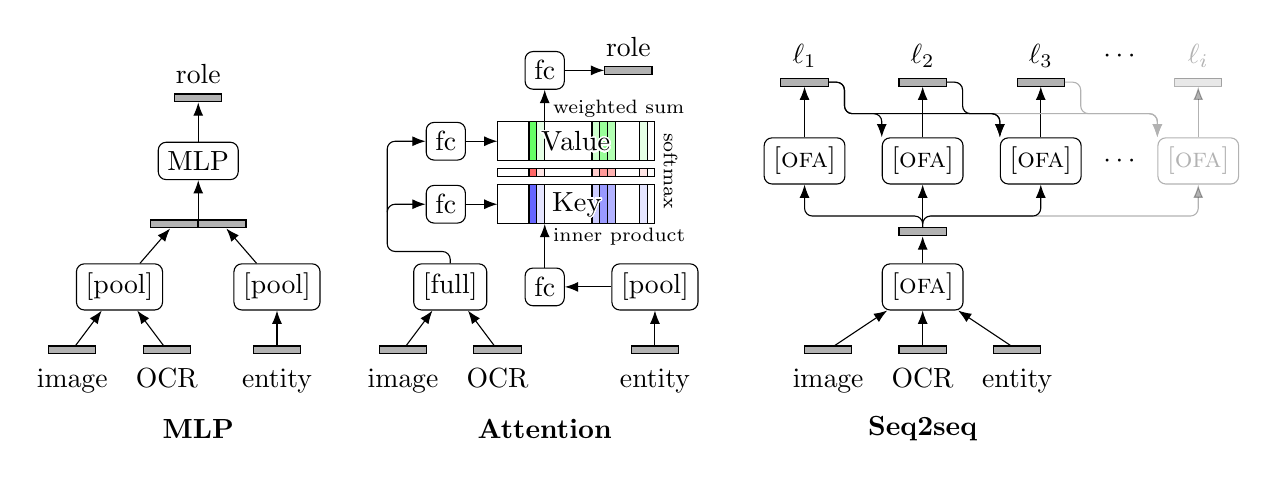
\begin{tikzpicture}[
			vector/.style={draw, rectangle, fill=black!30, inner sep=0mm, minimum width=6mm, minimum height=1mm},
			block/.style={draw, rectangle, rounded corners=0.1cm},
			value/.style={inner sep=0},
			text shadow/.code args={[#1]#2at#3(#4)#5}{
				\pgfkeysalso{/tikz/.cd,#1}%
				\foreach \angle in {0,5,...,359}{
					\node[#1,text=white] at ([shift={(\angle:.5pt)}] #4){#5};
				}
			},
		]
	\begin{scope}[shift={(0, 0)}]
		\node at (2.5, -0.5) {\textbf{MLP}};
		\node[vector] (vimage)  at (0.9, 0.5) {};
		\node[vector] (vocr)    at (2.1, 0.5) {};
		\node[vector] (ventity) at (3.5, 0.5) {};

		\node[below=0mm of vimage,  anchor=north] {\strut image};
		\node[below=0mm of vocr,    anchor=north] {\strut OCR};
		\node[below=0mm of ventity, anchor=north] {\strut entity};

		\node[block] (encmeme)   at (1.5, 1.3) {\encoder[pool]};
		\node[block] (encentity) at (3.5, 1.3) {\encoder[pool]};
		\draw[arrow] (vimage)  -- (encmeme);
		\draw[arrow] (vocr)    -- (encmeme);
		\draw[arrow] (ventity) -- (encentity);

		\node[vector, anchor=east] (embedmeme)   at (2.5, 2.1) {};
		\node[vector, anchor=west] (embedentity) at (2.5, 2.1) {};
		\draw[arrow] (encmeme) -- (embedmeme);
		\draw[arrow] (encentity) -- (embedentity);

		\node[block] (mlp)   at (2.5, 2.9) {MLP};
		\draw[arrow] (embedmeme.north east) -- (mlp);

		\node[vector] (vrole) at (2.5, 3.7) {};
		\node[above=0mm of vrole, anchor=south] {role};
		\draw[arrow] (mlp) -- (vrole);
	\end{scope}

	\begin{scope}[shift={(6.3, 2.6)}]
		\node at (0.6, -3.1) {\textbf{Attention}};
		\node (mk) at (0.12, -0.25) {};
		\node (mv) at (0.12, 0.55) {};
		\draw (0, -0.5) rectangle (2, 0);
		\draw (0, 0.3) rectangle (2, 0.8);

		\draw (0, 0.1) rectangle (2, 0.2);
		\node[rotate=270] at (2.2, 0.17) {\scriptsize softmax};
		\draw[fill=red!60] (0.4, 0.1) rectangle (0.5, 0.2);
		\draw[fill=red!10] (0.5, 0.1) rectangle (0.6, 0.2);
		\draw[fill=red!20] (1.2, 0.1) rectangle (1.3, 0.2);
		\draw[fill=red!40] (1.3, 0.1) rectangle (1.4, 0.2);
		\draw[fill=red!30] (1.4, 0.1) rectangle (1.5, 0.2);
		\draw[fill=red!10] (1.8, 0.1) rectangle (1.9, 0.2);

		\draw[fill=green!60] (0.4, 0.3) rectangle (0.5, 0.8);
		\draw[fill=green!10] (0.5, 0.3) rectangle (0.6, 0.8);
		\draw[fill=green!20] (1.2, 0.3) rectangle (1.3, 0.8);
		\draw[fill=green!40] (1.3, 0.3) rectangle (1.4, 0.8);
		\draw[fill=green!30] (1.4, 0.3) rectangle (1.5, 0.8);
		\draw[fill=green!10] (1.8, 0.3) rectangle (1.9, 0.8);

		\draw[fill=blue!60] (0.4, -0.5) rectangle (0.5, 0);
		\draw[fill=blue!10] (0.5, -0.5) rectangle (0.6, 0);
		\draw[fill=blue!20] (1.2, -0.5) rectangle (1.3, 0);
		\draw[fill=blue!40] (1.3, -0.5) rectangle (1.4, 0);
		\draw[fill=blue!30] (1.4, -0.5) rectangle (1.5, 0);
		\draw[fill=blue!10] (1.8, -0.5) rectangle (1.9, 0);

		\node[text shadow={[align=center,text width=3cm] at (1,0.55) {Value}}] at (1,0.55) {Value};
		\node[text shadow={[align=center,text width=3cm] at (1,-0.25) {Key}}] at (1,-0.25) {Key};

		\begin{scope}[shift={(-2.5, -2.6)}]
			\node[vector] (vimage)  at (1.3, 0.5) {};
			\node[vector] (vocr)    at (2.5, 0.5) {};
			\node[vector] (ventity) at (4.5, 0.5) {};

			\node[below=0mm of vimage,  anchor=north] {\strut image};
			\node[below=0mm of vocr,    anchor=north] {\strut OCR};
			\node[below=0mm of ventity, anchor=north] {\strut entity};

			\node[block] (encmeme)   at (1.9, 1.3) {\encoder[full]};
			\node[block] (encentity) at (4.5, 1.3) {\encoder[pool]};
			\node[block] (elinear)   at (3.1, 1.3) {fc};

			\draw[arrow] (vimage)  -- (encmeme);
			\draw[arrow] (vocr)    -- (encmeme);
			\draw[arrow] (ventity) -- (encentity);
			\draw[arrow] (encentity) -- (elinear);
		\end{scope}

		\coordinate (inter) at (-1.4, -0.85);
		\coordinate (tkey) at (0, -0.25);
		\coordinate (ukey) at (1, -0.5);
		\coordinate (tval) at (0, 0.55);
		\coordinate (uval) at (1, 0.8);

		\node[block, left=4mm of tkey, anchor=east] (klinear) {fc};
		\node[block, left=4mm of tval, anchor=east] (vlinear) {fc};

		\draw[rounded corners=1mm, arrow] (elinear) -- (elinear|-ukey);
		\draw[rounded corners=1mm, arrow] (encmeme) -- (encmeme|-inter) -- (inter) -- (inter|-tkey) -- (klinear);
		\draw[rounded corners=1mm, arrow] ($(inter) + (0, 5mm)$) -- (inter|-tval) -- (vlinear);

		\draw[arrow] (klinear) -- (tkey);
		\draw[arrow] (vlinear) -- (tval);

		\node[value, anchor=north west, yshift=-0.5mm] at (ukey-|elinear) {\scriptsize\kern1mm\relax inner product};
		\node[value, anchor=south west, yshift=0.5mm] at (uval-|elinear) {\scriptsize\kern1mm\relax weighted sum};

		\coordinate[above=6.5mm of uval] (top);
		\node[block] (linear) at (top-|elinear) {fc};
		\node[vector, right=5mm of linear, anchor=west] (vrole) {};
		\node[above=0mm of vrole, anchor=south] {role};
		\draw[arrow] (uval-|elinear) -- (linear);
		\draw[arrow] (linear) -- (vrole);
	\end{scope}

	\begin{scope}[shift={(9.2, 0)}]
		\node at (2.5, -0.5) {\textbf{Seq2seq}};
		\node[vector] (vimage)  at (1.3, 0.5) {};
		\node[vector] (vocr)    at (2.5, 0.5) {};
		\node[vector] (ventity) at (3.7, 0.5) {};

		\node[below=0mm of vimage,  anchor=north] {\strut image};
		\node[below=0mm of vocr,    anchor=north] {\strut OCR};
		\node[below=0mm of ventity, anchor=north] {\strut entity};

		\node[block] (enc)   at (2.5, 1.3) {\encoder[\textsc{ofa}]};
		\draw[arrow] (vimage)  -- (enc);
		\draw[arrow] (vocr)    -- (enc);
		\draw[arrow] (ventity) -- (enc);

		\node[vector] (embed)   at (2.5, 2) {};
		\draw[arrow] (enc) -- (embed);

		\coordinate (inter) at (2.5, 2.2);

		\foreach \i/\x/\f in {1/1/1, 2/2.5/1, 3/4/1, i/6/0.3}{
			\begin{scope}[opacity=\f]
				\node[block] (dec\i)   at (\x, 2.9) {\decoder[\textsc{ofa}]};
				\draw[arrow, rounded corners=1mm] (embed) -- (inter) -- (inter-|dec\i) -- (dec\i);
				\node[vector] (vrole\i) at (\x, 3.9) {};
				\coordinate (vn\i) at ($(vrole\i.east) + (2mm, 0)$);
				\node[above=0mm of vrole\i, anchor=south] (role\i) {\(\ell_\i\)};
				\draw[arrow] (dec\i) -- (vrole\i);
			\end{scope}
		}
	\end{scope}
	\node at ($(role3)!0.5!(rolei)$) {\(\cdots\)};
	\node at ($(dec3)!0.5!(deci)$) {\(\cdots\)};
	\coordinate (top) at (2.5, 3.5);
	\draw[arrow, rounded corners=1mm, black!30] (vrole2.east) -- (vn2) -- (vn2|-top) -- (top-|deci.150) -- (deci.150);
	\draw[arrow, rounded corners=1mm, black!30] (vrole3.east) -- (vn3) -- (vn3|-top) -- (top-|deci.150) -- (deci.150);
	\draw[arrow, rounded corners=1mm] (vrole1.east) -- (vn1) -- (vn1|-top) -- (top-|dec2.150) -- (dec2.150);
	\draw[arrow, rounded corners=1mm] (vrole1.east) -- (vn1) -- (vn1|-top) -- (top-|dec3.150) -- (dec3.150);
	\draw[arrow, rounded corners=1mm] (vrole2.east) -- (vn2) -- (vn2|-top) -- (top-|dec3.150) -- (dec3.150);
\end{tikzpicture}

	\caption{%
	    Our three classifiers.
	    Note that each classifier uses a different combination of encoders.
	    MLP is used with \encoder[pool], Attention requires \encoder[full], while Seq2seq requires an \encoder[\textsc{ofa}]--\decoder[\textsc{ofa}] pair.
	}
	\label{fig:models}
\end{figure*}

We now describe how we use the encoded text and images for semantic role labeling.

\subsection{Classification}
\label{sec:classification}
We experiment with three different methods to classify a \((\text{meme}, \text{entity})\) pair, depending on what kind of representation we get from the encoder.
The representation of the meme is composed of the image's representation along with the encoded caption's OCR, and any extra features such as the list of entities related to the meme.
For ease of notation, we group under ``OCR'' all extra features which were extracted from the meme, and we refer to them using a single variable \(o = (\text{OCR}, \text{caption, }\dotsc)\). Image features are referred to by  \(i\) and the encoded list of entities by  \(e\).
All classifiers are illustrated in Figure~\ref{fig:models}.

\paragraph{Multilayer perceptron (MLP)}
When the output of the encoder is of fixed size, we use a 2-layers MLP classifier.
The input of the classifier is made from the encoding of the OCR, image and entity.
The representation of the entity is obtained using the same transformer used to process the OCR.
The output of the model is a softmax on the four possible roles:
\begin{equation*}
	P(r\mid o, i, e) \propto \exp \operatorname{MLP}\left(\begin{bmatrix}\encoder[pool](o, i)\\\encoder[pool](e)\end{bmatrix}\right)_r.
\end{equation*}
This model is trained using a standard cross-entropy loss.
Depending on the encoder, we either train the MLP alone, or the MLP and the encoder jointly.

\paragraph{Attention}
When the representations of the OCR and image are not pooled along the sequence's length, we use an attention mechanism.
In this case, the query of the attention is the entity we wish to classify, while the memory is built from a concatenation of the image and OCR encoded by CLIP or VisualBERT:
\begin{align*}
	\alpha_j & \propto \exp \left( \encoder[pool](e)\transpose{} \bm{W}_k \encoder[full](o, i)_j \right), \\
	\bm{a} & = \operatorname{ReLU}\left(\sum_j \alpha_j \bm{W}_v \encoder[full](o, i)_j\right),
\end{align*}
where \(\bm{W}_k\) and \(\bm{W}_v\) are parameters used to project the encoded meme for use as attention key and value.
We classify the attention output \(\bm{a}\), using a softmax layer \(P(r\mid o, i, e) \propto \exp(\bm{W}_p \bm{a})_r\).

Since the encoders already use positional embeddings, we do not add this information to our classifier's attention.
However, we do use segment embeddings to distinguish the vectors encoding the image, OCR or entity list in the encoder's output. We use different MLP layers depending on whether a vector correspond to an input image, OCR or entity list.
This model is also trained by minimizing the cross-entropy with gold labels.

\paragraph{Seq2seq}
When using an OFA encoder, we also attempt to stay in the sequence to sequence framework and train the model to generate the class labels.
In this case, if we denote the label's tokens by \(\bm{\ell}\), the model is trained to maximize the likelihood that the meme \((o, i)\) has the gold target \(\bm{\ell}\):
\begin{equation*}
	P(\ell_k \mid \bm{\ell}_{<k}, o, i) \propto \decoder[ofa](\encoder[ofa](o, i), \bm{\ell}_{<k})_{\ell_k},
\end{equation*}
where \(\bm{\ell}_{<k} = [\ell_1, \ell_2, \dotsc, \ell_{k-1}]\transpose\) refers to the list of previous tokens.
To evaluate this model, the log-likelihood of the possible labels are summed along sequence length:
\begin{equation*}
	\hat{r} = \arg\,\max_r P(r \mid o, i) \propto \prod_k P(\ell^{(r)}_k \mid \ell^{(r)}_{<k}, o, i),
\end{equation*}
where \(\bm{\ell}^{(r)}\) designates the list of tokens for the label \(r\), such as \([\texttt{vil}, \texttt{lain}]\transpose\).


\paragraph{Additional features}
As explained in Section \ref{sec:literature}, our task is quite different from most multimodal tasks on which the encoders were trained; it is much more abstract and requires a lot of additional background knowledge.
Thus, when using CLIP and VisualBERT, we add supplementary features as input to the classification model (MLP and attention).

We add as textual features the list of entities associated with the meme, this list is directly available in the dataset. We encode the entities' names using the same encoder as the system (CLIP or VisualBERT).\footnote{We also experiment with adding generated captions as features. We generate them using an OFA model trained for automatic caption generation. However, the captions are very generic and descriptive; for example the entities names are not captured by the model. This features does not improve the systems, hence we do not further develop it in the results section.} We also add to the system the image features that were extracted using VGG, EfficientNET and FRCNN.
%The entities are encoded using SentenceTransformer \cite{reimers2019sentence}, with a Distil-Roberta model trained on paraphrasing.

\subsection{Dealing with Class Imbalance}
\label{sec:subsampling}
The dataset faces a large class imbalance, with the class \texttt{other} being over-represented (78\% in the train set) and classes \texttt{hero} and \texttt{victim} consisting of only 2.7\% and 5.2\% of the train set respectively.
Thus, training on the raw dataset might lead to overfitting and over-predicting the majority class.
Moreover, recall that the evaluation metric is Macro-\fone{}, which weighs each class equally; hence the importance of solving the class imbalance issue.

Our first solution was to weight labels in the loss. This loss penalisation led to poor performances; we suspect this is due to the working of the optimization algorithm we used.
Adam and its variants estimate the distribution of the gradients using exponential moving averages; these estimates are faulty when the magnitude of the loss changes often.

A common strategy is over-sampling the low-frequency classes and under-sampling the high-frequency ones. Each (meme, entity) pair is dropped with a pre-defined probability, following various class sampling strategies.
We evaluated 6 different sampling strategies illustrated in Figure~\ref{fig:sampling}:
\begin{description}
	\item[\textsl{Micro}] does not subsample.
    This optimize the Micro-\fone{}, which puts more weight on samples labeled \texttt{other} due to their sheer number.
	\item[\textsl{Macro}] subsamples memes such that the label distribution is uniform.
    This implies dropping a large amount of \texttt{other} samples in order to lower their frequency.
	\item[\textsl{In-between}] is a compromise between \textsl{micro} and \textsl{macro}, balancing between matching the evaluation loss and seeing a more diverse set of samples.
	\item[\textsl{Interpolate}] drifts from \textsl{micro} to \textsl{macro} during training.
	For the first epoch, the memes are sampled according to the empirical distribution (\textsl{micro}); while the last epoch is sampled to have a uniform label distribution (\textsl{macro}).
	\item[\textsl{Cycle}] alternates between \textsl{micro} and \textsl{macro} (2-epoch \textsl{short cycle}) or between \textsl{micro}, \textsl{macro} and two different \textsl{in-between} (4-epoch \textsl{long cycle}).
\end{description}

For the last two strategies, the sampling rates are updated at the end of each epoch during training.
In general, these \emph{dynamic} sampling strategies performed better than sampling strategies with a fixed rate for the whole training duration.

\begin{figure}
	\centering
	\NewDocumentCommand\distrib{m m m m m}{
	\pgfmathsetmacro{\xa}{1.25*(#3)}
	\pgfmathsetmacro{\xb}{1.25*(#3+#4)}
	\pgfmathsetmacro{\xc}{1.25*(#3+#4+#5)}
	\pgfmathsetmacro{\xd}{1.25}
	\coordinate (#1-a) at (#2, 0);
	\coordinate (#1-b) at (#2, \xa);
	\coordinate (#1-c) at (#2, \xb);
	\coordinate (#1-d) at (#2, \xc);
	\coordinate (#1-e) at (#2, \xd);
}

\NewDocumentCommand\drawRegion{m m m m m m}{
	\fill[Set3-#6] (#1-0-#4)
		\foreach \i in {#2}{ -- (#1-\i-#4)}
		\foreach \i in {#3}{ -- (#1-\i-#5)}
		-- cycle;
}

\NewDocumentCommand\drawPlot{m m m}{
	\drawRegion{#1}{#2}{#3}{a}{b}{A};
	\drawRegion{#1}{#2}{#3}{b}{c}{D};
	\drawRegion{#1}{#2}{#3}{c}{d}{C};
	\drawRegion{#1}{#2}{#3}{d}{e}{B};
}

\begin{tikzpicture}[
			legend/.style={anchor=north, inner sep=0},
			braced/.style={decorate,decoration={brace,amplitude=2}},
		]
	\begin{scope}[shift={(0.375, 0)}]
		\distrib{micro-0}{0   }{0.027121160214685396}{0.13857485440219253}{0.05195843325339728}
		\distrib{micro-1}{0.25}{0.027121160214685396}{0.13857485440219253}{0.05195843325339728}
		\node[legend] at (0.125, 0) {\strut\small micro};
		\drawPlot{micro}{0,1}{1,0}
	\end{scope}

	\begin{scope}[shift={(1.7, 0)}]
		\distrib{affine-0}{0  }{0.081}{0.165}{0.099}
		\distrib{affine-1}{0.25}{0.081}{0.165}{0.099}
		\node[legend] at (0.125, 0) {\strut\small in-between};
		\drawPlot{affine}{0,1}{1,0}
	\end{scope}

	\begin{scope}[shift={(3.025, 0)}]
		\distrib{macro-0}{0   }{0.25}{0.25}{0.25}
		\distrib{macro-1}{0.25}{0.25}{0.25}{0.25}
		\node[legend] at (0.125, 0) {\strut\small macro};
		\drawPlot{macro}{0,1}{1,0}
	\end{scope}

	\begin{scope}[shift={(0, -2)}]
		\distrib{interpolate-0}{0  }{0.027121160214685396}{0.13857485440219253}{0.05195843325339728}
		\distrib{interpolate-1}{1}{0.25}{0.25}{0.25}
		\node[legend] at (0.5, 0) {\strut\small interpolate};
		\drawPlot{interpolate}{0,1}{1,0}
	\end{scope}

	\begin{scope}[shift={(2, -2)}]
		\foreach \a in {0,0.125,...,0.875}{
			\pgfmathsetmacro{\x}{int(mod(8*\a, 2))}
			\pgfmathsetmacro{\b}{\a+0.125}
			\ifthenelse{\x=0}{
				\distrib{short-\x-0}{\a}{0.027121160214685396}{0.13857485440219253}{0.05195843325339728}
				\distrib{short-\x-1}{\b}{0.027121160214685396}{0.13857485440219253}{0.05195843325339728}
			}{
				\distrib{short-\x-0}{\a}{0.25}{0.25}{0.25}
				\distrib{short-\x-1}{\b}{0.25}{0.25}{0.25}
			}
			\drawPlot{short-\x}{0,1}{1,0}
		}
		\node[legend] at (0.5, 0) {\strut\small short cycle};
	\end{scope}

	\begin{scope}[shift={(4, -2)}]
		\foreach \a in {0,0.125,...,1.475}{
			\pgfmathsetmacro{\n}{int(8*\a)}
			\pgfmathsetmacro{\x}{int(mod(8*\a, 4))}
			\pgfmathsetmacro{\b}{\a+0.125}
			\ifthenelse{\x=0}{
				\distrib{long-\n-0}{\a}{0.176}{0.213}{0.184}
				\distrib{long-\n-1}{\b}{0.176}{0.213}{0.184}
			}{
			\ifthenelse{\x=1}{
				\distrib{long-\n-0}{\a}{0.027121160214685396}{0.13857485440219253}{0.05195843325339728}
				\distrib{long-\n-1}{\b}{0.027121160214685396}{0.13857485440219253}{0.05195843325339728}
			}{
			\ifthenelse{\x=2}{
				\distrib{long-\n-0}{\a}{0.077}{0.163}{0.096}
				\distrib{long-\n-1}{\b}{0.077}{0.163}{0.096}
			}{
				\distrib{long-\n-0}{\a}{0.25}{0.25}{0.25}
				\distrib{long-\n-1}{\b}{0.25}{0.25}{0.25}
			}}}
			\drawPlot{long-\n}{0,1}{1,0}
		}
		\node[legend] at (0.75, 0) {\strut\small long cycle};
	\end{scope}

	\draw[arrow] ($(long-0-0-e) + (0, 1mm)$) -- ($(long-11-1-e) + (0, 1mm)$) node[midway, anchor=south, yshift=-1mm] {\footnotesize training time};

	%\draw[braced] (macro-1-b) -- (macro-1-a) node[midway, anchor=west, xshift=0.5mm] {\footnotesize heroes};
	%
	%\draw (macro-1-c) -- ($(macro-1-c) + (1mm, 0)$);
	%\draw (macro-1-b) -- ($(macro-1-b) + (1mm, 0)$);
	%\draw[braced] ($(macro-1-c) + (1mm, 0)$) -- ($(macro-1-b) + (1mm, 0)$) node[midway, anchor=west, xshift=0.5mm] {\footnotesize villains};
	%
	%\draw[braced] (macro-1-d) -- (macro-1-c) node[midway, anchor=west, xshift=0.5mm] {\footnotesize victims};
	%
	%\draw (macro-1-e) -- ($(macro-1-e) + (1mm, 0)$);
	%\draw (macro-1-d) -- ($(macro-1-d) + (1mm, 0)$);
	%\draw[braced] ($(macro-1-e) + (1mm, 0)$) -- ($(macro-1-d) + (1mm, 0)$) node[midway, anchor=west, xshift=0.5mm] {\footnotesize others};

	\draw[braced] (macro-1-b) -- (macro-1-a) node[midway, anchor=west, xshift=0.3mm] {\footnotesize\strut heroes};
	\draw[braced] (macro-1-c) -- (macro-1-b) node[midway, anchor=west, xshift=0.3mm] {\footnotesize\strut villains};
	\draw[braced] (macro-1-d) -- (macro-1-c) node[midway, anchor=west, xshift=0.3mm] {\footnotesize\strut victims};
	\draw[braced] (macro-1-e) -- (macro-1-d) node[midway, anchor=west, xshift=0.3mm] {\footnotesize\strut others};
\end{tikzpicture}

	\caption{
		Target frequencies of the various strategies during training.
		The \textsl{micro} strategy corresponds to using the empirical class distribution in the dataset, that is hero 2.7\%, villain 13.9\%, victim 5.2\% and other 78.2\%.}
	\label{fig:sampling}
\end{figure}

\subsection{Ensembling}
\label{sec:ensembling}
In order to further improve our results, we build several ensemble of our models.
We filter-out models with a low validation macro-\fone{} and experiment with several ensembling techniques.
Due to the small size of the dataset, we did not create an additional split to evaluate our ensembling approach.
In this context, overfitting the validation set is a risk.
Two of the ensembling methods we evaluate are therefore non-parametric.
These non-parametric strategies take the average or the median probability assigned to each class by all models.

Preliminary results indicate that training a linear model to weight the output of our various models is tedious and does not improve over non-parametric strategies.
We therefore turn towards gradient boosted trees \citep{gradient_boosting} trained by XGBoost \citep{xgboost}.
XGBoost builds an ensemble of decision trees, whose internal nodes correspond to conditions on our models' output, and whose leaves correspond to a predicted semantic role.
Boosted trees have the potential to outperform non-parametric methods by better capturing the scale of various models' output, however it has the downside of being very prone to overfitting.

\section{Results}
\label{sec:results}

\subsection{Experimental process}
The train set consists of 17\,514 (meme, entity) pairs, the validation set 2\,069 pairs and the test set 2\,433 pairs. We did all the training on the datasets from the two domains, \textsc{covid}-19 and US politics jointly. The test set contains examples from both domains.
The evaluation is done with Macro-\fone{} score; the OCR and the list of entities are provided along with the image of the meme. We run all experiments 5 times to check for the robustness of results and perform statistical testing.


For CLIP, we use the biggest \texttt{L/14} CLIP-ViT model built on the Vision Transformers \cite{dosovitskiy2020image}. Both preliminary self-supervised fine-tuning and fine-tuning while doing the classification failed. This is probably due to the size and the format of the shared task dataset, much smaller and quite different from the training data of the pre-trained model; any fine-tuning leads the model to forget the knowledge it learned during pre-training. Consequently, we freeze all layers and tune only the classifier, with the architectures described in Section~\ref{sec:models}.  

For VisualBERT, we fine-tune the \texttt{visualbert-vcr-coco-pre} model trained on caption generation and visual commonsense reasoning.

For OFA \encoder[pool] with an MLP classifier, we obtained better results by fine-tuning the whole model from the \texttt{vqa\_large\_best} checkpoint\footnote{This refers to an OFA model pre-trained on 8 tasks then fine-tuned on VQA from the official OFA repository.} using a small 0.1 label smoothing and feeding the OCR and entity both to the encoder -- along with the image -- and to the decoder.
Our OFA seq2seq model follows the same setup using the \texttt{ofa\_base} checkpoint.

In the dataset, several entities are associated with more that one label.
As this situation is infrequent, we consider the small amount of samples with multiple labels does not warrant a full-fledged multi-label classification setup.
Thus, our models output a single categorical distribution. When multiple labels ought to be predicted for an entity (the entity appears twice in the list of entities associated with the meme), we predict them in order of likelihood.


\subsection{Quantitative results}


\begin{table}[t]
	\centering
	\begin{tabular}{l l r r}
\toprule
	\multirow{2}{*}{Encoder} & \multirow{2}{*}{Classifier} & \multicolumn{2}{c}{Macro-\fone{}} \\
	\cmidrule(lr){3-4}
	& & \multicolumn{1}{c}{mean} & \multicolumn{1}{c}{std} \\
\midrule
	OFA & MLP & 44.6 & 0.5 \\
	OFA & Seq2seq & 44.0 & 0.9 \\
\midrule
	CLIP & MLP & \textbf{47.0} & 0.5 \\
	CLIP$^*$ & Attention & 42.3 & 1.7 \\
\midrule
    VisualBERT$^*$ & MLP & 43.1 & 0.2 \\
	VisualBERT$^*$ & Attention & 42.3 & 1.8 \\
\midrule
	\multicolumn{2}{l}{Ensemble mean   } & 47.9 & - \\
	\multicolumn{2}{l}{Ensemble median } & 47.5 & - \\
	\multicolumn{2}{l}{Ensemble XGBoost} & 47.6 & - \\
\midrule
	\multicolumn{2}{l}{Challenge's top score} & 58.7 & - \\
	\multicolumn{2}{l}{Human} & 65.5 & 4.6 \\
\bottomrule
\end{tabular}

	\caption{Comparison of the best systems with the different encoders and classification architectures. All systems are run 5 times with 25 epochs. Encoders with a $^*$ in exponent are augmented with the list of entities as feature.}
	\label{tab:models}	
\end{table}

\begin{table}[t]
	\centering
	\begin{tabular}{l r r}
\toprule
	\multirow{2}{*}{Sampling} & \multicolumn{2}{c}{Macro-\fone{}} \\
	\cmidrule(lr){2-3}
	 & \multicolumn{1}{c}{mean} & \multicolumn{1}{c}{std} \\
\midrule
	micro & 38.3 & 1.0 \\
	in-between & 44.1 & 0.3 \\
	macro & 42.3 & 0.6 \\
	interpolate & 46.3 & 0.8 \\
    short cycle & \textbf{47.0} & 0.5 \\
	long cycle & 46.5 & 0.5 \\
\bottomrule
\end{tabular}

	\caption{Sampling results with the CLIP model and MLP classifier, with 500 batch per epoch.}
	\label{tab:sampling}
\end{table}

\paragraph{Classifier results.}
Table~\ref{tab:models} compares our main models on the \textsc{constraint}'22 test set.
We measure the statistical significance of our results using a one-sided Welch's unequal variances \(t\)-test \citep{welch} under the null hypothesis that the macro-\fone{} are equals.
Some hyperparameters are optimized on a per-model basis. In particular,  using the list of entities as additional feature improves the performance for VisualBERT and CLIP-attention but not for our best CLIP-MLP model.

A CLIP \encoder[pool] together with an MLP classifier reached the best performances among our non-ensembling model pool, significantly (\(p<0.0004\)) improving over the OFA MLP combination.
Using the unpooled features of the transformers (\encoder[full]) with an attention classifier underperform compared to the \encoder[pool]+MLP approach.
However this difference is not significant in the case of VisualBERT (\(p<0.3\)).
In particular, attention-based approaches have more variance than their MLP counterpart.
The OFA seq2seq model reaches performances within the error margin of the OFA MLP model (\(p<0.14\)), which is not surprising since the two models are relatively close.
The gap between VisualBERT and OFA is somewhat significant with \(p\)-values between 0.001 and 0.07 depending on the pairwise comparison.
As expected, ensembling leads to the best result, regardless of the ensembling strategy; human annotators far exceed current model performances.
We further develop human annotation in Section \ref{sec:discussion}.

\paragraph{Sampling results.}
Table~\ref{tab:sampling} compares the different sampling strategies represented in Figure~\ref{fig:sampling} for training a CLIP encoder with MLP model. As expected, using the empirical class distribution (\textsl{micro} strategy) leads to the worse score.
While the \textsl{macro} strategy is in theory what we should maximise to improve the Macro-\fone{}, it is second worst among all strategies.
The dynamic strategies, which use evolving sampling frequencies during training clearly outperform static strategies.
In particular, for training CLIP, the \textsl{short cycle} strategy outperforms the other ones, but the difference with \textsl{long cycle} and \textsl{interpolate} is not statistically significant (\(p\)-values > 0.05).
We observe similar tendencies with systems based on OFA and VisualBERT, with a slight advantage to the \textsl{interpolate} strategy over the \textsl{cycling} ones for the former.

Despite the different subsampling strategies, the per-class performances vary widely, see for example the results for the CLIP MLP model with a \textsl{short cycling} subsampling strategy:
\begin{center}
\begin{tabular}{l r r r r}
\toprule
\% & hero & villain & victim & other \\
\midrule
\fone{} & 20 & 50 & 33 & 84 \\
Precision & 15 & 46 & 26 & 90 \\
Recall & 33 & 56 & 45 & 79 \\
\bottomrule
\end{tabular}
\end{center}
We observe similar results with all hyperparameter combination.
These performances somewhat follow the empirical distribution of the classes, with the rarest class \texttt{hero} having the worst performance, and \texttt{victim} being not much better.
This makes us consider sub-sampling \texttt{other} even below 25\%.
However, this observation-inspired ``\textsl{super-macro}'' strategy did not prove successful, reaching an average Macro-\fone{} or 40.0, higher than the \textsl{micro} strategy but lower than the \textsl{macro} one.

\subsection{Qualitative analysis}
\begin{figure}
	\centering
	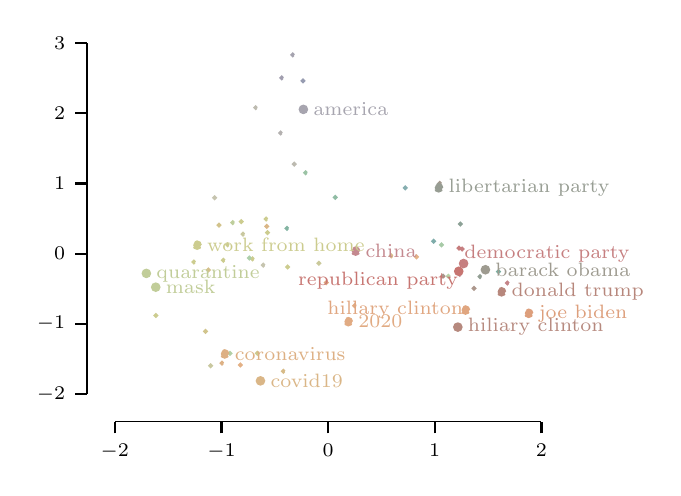
\begin{tikzpicture}
    \begin{axis}[
            enlargelimits=false,
            separate axis lines,
            semithick,
            axis x line*=bottom,
            axis x line shift=10pt,
            axis y line*=left,
            axis y line shift=10pt,
            every axis/.append style={thick},
            tick style={thick, black},
            tick align=outside,
            width=70mm,
            xmin=-2,
            xmax=2,
            ymin=-2,
            ymax=3,
            xtick={-2, -1, ..., 2},
            ytick={-2, -1, ..., 3},
            every tick label/.append style={font=\scriptsize},
    	]
\addplot+ [draw={black!20!Set3-A!59!Set3-D}, only marks, mark=*, mark size=0.2mm, mark options={fill={black!20!Set3-A!59!Set3-D}},
    	] coordinates {
(1.0778651600293996, -0.320872764196061)
};
\addplot+ [draw={black!20!Set3-B!84!Set3-D}, only marks, mark=*, mark size=0.2mm, mark options={fill={black!20!Set3-B!84!Set3-D}},
    	] coordinates {
(-1.1224384998993704, -0.23145139685532382)
};
\addplot+ [draw={black!20!Set3-C!89!Set3-A}, only marks, mark=*, mark size=0.2mm, mark options={fill={black!20!Set3-C!89!Set3-A}},
    	] coordinates {
(-0.23575493633421607, 2.462143684586866)
};
\addplot+ [draw={black!20!Set3-B!71!Set3-D}, only marks, mark=*, mark size=0.2mm, mark options={fill={black!20!Set3-B!71!Set3-D}},
    	] coordinates {
(-0.5746261726075611, 0.3895394033163904)
};
\addplot+ [draw={black!20!Set3-A!82!Set3-C}, only marks, mark=*, mark size=0.2mm, mark options={fill={black!20!Set3-A!82!Set3-C}},
    	] coordinates {
(0.9892194921595016, 0.17768224606482086)
};
\addplot+ [draw={black!20!Set3-A!50!Set3-B}, only marks, mark=*, mark size=0.2mm, mark options={fill={black!20!Set3-A!50!Set3-B}},
    	] coordinates {
(1.1277258373176067, -0.32355060185167483)
};
\addplot+ [draw={black!20!Set3-B!64!Set3-D}, only marks, mark=*, mark size=0.2mm, mark options={fill={black!20!Set3-B!64!Set3-D}},
    	] coordinates {
(-0.9947844374325617, -1.5607014445646492)
};
\addplot+ [draw={black!20!Set3-B!100!Set3-C}, only marks, mark=*, mark size=0.2mm, mark options={fill={black!20!Set3-B!100!Set3-C}},
    	] coordinates {
(-0.5813744733055675, 0.49272447220316257)
};
\addplot+ [draw={black!20!Set3-B!100!Set3-C}, only marks, mark=*, mark size=0.2mm, mark options={fill={black!20!Set3-B!100!Set3-C}},
    	] coordinates {
(-1.2586872422655546, -0.12023776301666363)
};
\addplot+ [draw={black!20!Set3-D!52!Set3-C}, only marks, mark=*, mark size=0.2mm, mark options={fill={black!20!Set3-D!52!Set3-C}},
    	] coordinates {
(1.2345554928547289, -0.2944689627726048)
};
\addplot+ [draw={black!20!Set3-B!100!Set3-C}, only marks, mark=*, mark size=0.2mm, mark options={fill={black!20!Set3-B!100!Set3-C}},
    	] coordinates {
(-0.814198430304801, 0.4554229601435057)
};
\addplot+ [draw={black!20!Set3-A!93!Set3-B}, only marks, mark=*, mark size=0.2mm, mark options={fill={black!20!Set3-A!93!Set3-B}},
    	] coordinates {
(1.5976147630179844, -0.2555828656732836)
};
\addplot+ [draw={black!20!Set3-A!78!Set3-B}, only marks, mark=*, mark size=0.2mm, mark options={fill={black!20!Set3-A!78!Set3-B}},
    	] coordinates {
(0.06660838084954968, 0.8024485852387251)
};
\addplot+ [draw={black!20!Set3-C!65!Set3-B}, only marks, mark=*, mark size=0.2mm, mark options={fill={black!20!Set3-C!65!Set3-B}},
    	] coordinates {
(-0.3180504861393114, 1.2757557064501086)
};
\addplot+ [draw={black!20!Set3-A!57!Set3-D}, only marks, mark=*, mark size=0.2mm, mark options={fill={black!20!Set3-A!57!Set3-D}},
    	] coordinates {
(1.3688017771175727, -0.495081788090659)
};
\addplot+ [draw={black!20!Set3-B!77!Set3-D}, only marks, mark=*, mark size=0.2mm, mark options={fill={black!20!Set3-B!77!Set3-D}},
    	] coordinates {
(-0.4198826003314074, -1.6762289016965282)
};
\addplot+ [draw={black!20!Set3-A!70!Set3-B}, only marks, mark=*, mark size=0.2mm, mark options={fill={black!20!Set3-A!70!Set3-B}},
    	] coordinates {
(-0.2105520536984745, 1.1526050569114412)
};
\addplot+ [draw={black!20!Set3-C!64!Set3-B}, only marks, mark=*, mark size=0.2mm, mark options={fill={black!20!Set3-C!64!Set3-B}},
    	] coordinates {
(-0.6786950299396077, 2.0798832405102208)
};
\addplot+ [draw={black!20!Set3-B!100!Set3-C}, only marks, mark=*, mark size=0.2mm, mark options={fill={black!20!Set3-B!100!Set3-C}},
    	] coordinates {
(-0.9426151223908349, 0.12606274620047478)
};
\addplot+ [draw={black!20!Set3-C!73!Set3-B}, only marks, mark=*, mark size=0.2mm, mark options={fill={black!20!Set3-C!73!Set3-B}},
    	] coordinates {
(-0.4445141354196121, 1.7202312729163853)
};
\addplot+ [draw={black!20!Set3-B!100!Set3-C}, only marks, mark=*, mark size=0.2mm, mark options={fill={black!20!Set3-B!100!Set3-C}},
    	] coordinates {
(-0.5676999038611469, 0.30063492799980096)
};
\addplot+ [draw={black!20!Set3-B!88!Set3-D}, only marks, mark=*, mark size=0.2mm, mark options={fill={black!20!Set3-B!88!Set3-D}},
    	] coordinates {
(-1.0229691376249204, 0.4065280091654615)
};
\addplot+ [draw={black!20!Set3-B!59!Set3-A}, only marks, mark=*, mark size=0.2mm, mark options={fill={black!20!Set3-B!59!Set3-A}},
    	] coordinates {
(-0.9192867531408428, -1.4215159043983847)
};
\addplot+ [draw={black!20!Set3-B!100!Set3-C}, only marks, mark=*, mark size=0.2mm, mark options={fill={black!20!Set3-B!100!Set3-C}},
    	] coordinates {
(-1.6137216529633382, -0.8814557755619525)
};
\addplot+ [draw={black!20!Set3-B!58!Set3-C}, only marks, mark=*, mark size=0.2mm, mark options={fill={black!20!Set3-B!58!Set3-C}},
    	] coordinates {
(-1.0637421186726348, 0.7953010620155614)
};
\addplot+ [draw={black!20!Set3-B!100!Set3-C}, only marks, mark=*, mark size=0.2mm, mark options={fill={black!20!Set3-B!100!Set3-C}},
    	] coordinates {
(-0.9817437020554485, -0.09452679524422053)
};
\addplot+ [draw={black!20!Set3-A!64!Set3-D}, only marks, mark=*, mark size=0.2mm, mark options={fill={black!20!Set3-A!64!Set3-D}},
    	] coordinates {
(1.047365650323786, 1.0005444450898708)
};
\addplot+ [draw={black!20!Set3-B!58!Set3-C}, only marks, mark=*, mark size=0.2mm, mark options={fill={black!20!Set3-B!58!Set3-C}},
    	] coordinates {
(-0.6073387927034177, -0.164374005126457)
};
\addplot+ [draw={black!20!Set3-B!100!Set3-C}, only marks, mark=*, mark size=0.2mm, mark options={fill={black!20!Set3-B!100!Set3-C}},
    	] coordinates {
(-0.7084832328653686, -0.07566908465785661)
};
\addplot+ [draw={black!20!Set3-B!74!Set3-D}, only marks, mark=*, mark size=0.2mm, mark options={fill={black!20!Set3-B!74!Set3-D}},
    	] coordinates {
(0.5925254502214553, -0.030765133450945104)
};
\addplot+ [draw={black!20!Set3-B!90!Set3-D}, only marks, mark=*, mark size=0.2mm, mark options={fill={black!20!Set3-B!90!Set3-D}},
    	] coordinates {
(-1.149107419934683, -1.1091759738390805)
};
\addplot+ [draw={black!20!Set3-B!77!Set3-C}, only marks, mark=*, mark size=0.2mm, mark options={fill={black!20!Set3-B!77!Set3-C}},
    	] coordinates {
(-1.1018682878830781, -1.5981065343454175)
};
\addplot+ [draw={black!20!Set3-B!100!Set3-C}, only marks, mark=*, mark size=0.2mm, mark options={fill={black!20!Set3-B!100!Set3-C}},
    	] coordinates {
(-0.6628281014890972, -1.4198513915624158)
};
\addplot+ [draw={black!20!Set3-A!62!Set3-B}, only marks, mark=*, mark size=0.2mm, mark options={fill={black!20!Set3-A!62!Set3-B}},
    	] coordinates {
(1.0632145683493364, 0.12463264204171531)
};
\addplot+ [draw={black!20!Set3-D!50!Set3-B}, only marks, mark=*, mark size=0.2mm, mark options={fill={black!20!Set3-D!50!Set3-B}},
    	] coordinates {
(0.8286753605845535, -0.045386252143634946)
};
\addplot+ [draw={black!20!Set3-B!56!Set3-D}, only marks, mark=*, mark size=0.2mm, mark options={fill={black!20!Set3-B!56!Set3-D}},
    	] coordinates {
(0.2479722260996187, -0.7425220814074434)
};
\addplot+ [draw={black!20!Set3-A!87!Set3-B}, only marks, mark=*, mark size=0.2mm, mark options={fill={black!20!Set3-A!87!Set3-B}},
    	] coordinates {
(-0.38524578475436927, 0.3604978919274511)
};
\addplot+ [draw={black!20!Set3-C!87!Set3-B}, only marks, mark=*, mark size=0.2mm, mark options={fill={black!20!Set3-C!87!Set3-B}},
    	] coordinates {
(-0.33187157171131876, 2.8318469895874987)
};
\addplot+ [draw={black!20!Set3-B!79!Set3-C}, only marks, mark=*, mark size=0.2mm, mark options={fill={black!20!Set3-B!79!Set3-C}},
    	] coordinates {
(-0.79724599518393, 0.2787258073474104)
};
\addplot+ [draw={black!20!Set3-D!65!Set3-C}, only marks, mark=*, mark size=0.2mm, mark options={fill={black!20!Set3-D!65!Set3-C}},
    	] coordinates {
(1.6813758412132773, -0.4192469523338091)
};
\addplot+ [draw={black!20!Set3-D!51!Set3-B}, only marks, mark=*, mark size=0.2mm, mark options={fill={black!20!Set3-D!51!Set3-B}},
    	] coordinates {
(-0.8215263506093641, -1.5865136617600732)
};
\addplot+ [draw={black!20!Set3-B!100!Set3-C}, only marks, mark=*, mark size=0.2mm, mark options={fill={black!20!Set3-B!100!Set3-C}},
    	] coordinates {
(-0.37973540440880676, -0.1896414921825977)
};
\addplot+ [draw={black!20!Set3-A!72!Set3-C}, only marks, mark=*, mark size=0.2mm, mark options={fill={black!20!Set3-A!72!Set3-C}},
    	] coordinates {
(0.7239113318163237, 0.9375827611097706)
};
\addplot+ [draw={black!20!Set3-D!70!Set3-C}, only marks, mark=*, mark size=0.2mm, mark options={fill={black!20!Set3-D!70!Set3-C}},
    	] coordinates {
(1.2565931881289851, 0.06540499605327234)
};
\addplot+ [draw={black!20!Set3-B!84!Set3-C}, only marks, mark=*, mark size=0.2mm, mark options={fill={black!20!Set3-B!84!Set3-C}},
    	] coordinates {
(-0.08631683045456374, -0.1383540460112504)
};
\addplot+ [draw={black!20!Set3-C!91!Set3-B}, only marks, mark=*, mark size=0.2mm, mark options={fill={black!20!Set3-C!91!Set3-B}},
    	] coordinates {
(-0.4345950546605853, 2.5045034102636623)
};
\addplot+ [draw={black!20!Set3-B!51!Set3-A}, only marks, mark=*, mark size=0.2mm, mark options={fill={black!20!Set3-B!51!Set3-A}},
    	] coordinates {
(-0.7377493552616028, -0.06288056840506015)
};
\addplot+ [draw={black!20!Set3-B!77!Set3-A}, only marks, mark=*, mark size=0.2mm, mark options={fill={black!20!Set3-B!77!Set3-A}},
    	] coordinates {
(-0.8936144053319472, 0.44196365189515)
};
\addplot+ [draw={black!20!Set3-A!75!Set3-D}, only marks, mark=*, mark size=0.2mm, mark options={fill={black!20!Set3-A!75!Set3-D}},
    	] coordinates {
(1.4243235019121223, -0.3261694214357488)
};
\addplot+ [draw={black!20!Set3-D!73!Set3-C}, only marks, mark=*, mark size=0.2mm, mark options={fill={black!20!Set3-D!73!Set3-C}},
    	] coordinates {
(1.2272530011651106, 0.07793172349994809)
};
\addplot+ [draw={black!20!Set3-A!80!Set3-D}, only marks, mark=*, mark size=0.2mm, mark options={fill={black!20!Set3-A!80!Set3-D}},
    	] coordinates {
(1.2400952960997131, 0.42218774922052144)
};
\addplot+ [draw={black!20!Set3-D!57!Set3-B}, only marks, mark=*, mark size=0.2mm, mark options={fill={black!20!Set3-D!57!Set3-B}},
    	] coordinates {
(-0.01720804832178509, -0.4116139591923109)
};
\addplot+ [draw={black!20!Set3-C!85!Set3-B}, only marks, mark=*, mark size=0.5mm, mark options={fill={black!20!Set3-C!85!Set3-B}}, nodes near coords, point meta=explicit symbolic,
            nodes near coords style = {anchor=west, font=\scriptsize},
    	] coordinates {
(-0.2315977874508688, 2.0557491689397835) [\textcolor{black!20!Set3-C!85!Set3-B}{america}]
};
\addplot+ [draw={black!20!Set3-B!82!Set3-A}, only marks, mark=*, mark size=0.5mm, mark options={fill={black!20!Set3-B!82!Set3-A}}, nodes near coords, point meta=explicit symbolic,
            nodes near coords style = {anchor=west, font=\scriptsize},
    	] coordinates {
(-1.7036153931873892, -0.2814987603212383) [\textcolor{black!20!Set3-B!82!Set3-A}{quarantine}]
};
\addplot+ [draw={black!20!Set3-D!68!Set3-A}, only marks, mark=*, mark size=0.5mm, mark options={fill={black!20!Set3-D!68!Set3-A}}, nodes near coords, point meta=explicit symbolic,
            nodes near coords style = {anchor=west, font=\scriptsize},
    	] coordinates {
(1.2163794606328924, -1.0468088006994418) [\textcolor{black!20!Set3-D!68!Set3-A}{hiliary clinton}]
};
\addplot+ [draw={black!20!Set3-D!58!Set3-B}, only marks, mark=*, mark size=0.5mm, mark options={fill={black!20!Set3-D!58!Set3-B}}, nodes near coords, point meta=explicit symbolic,
            nodes near coords style = {anchor=east, inner sep=0.2mm, font=\scriptsize},
    	] coordinates {
(1.2883141722762896, -0.8040364727850706) [\textcolor{black!20!Set3-D!58!Set3-B}{hillary clinton}]
};
\addplot+ [draw={black!20!Set3-A!72!Set3-D}, only marks, mark=*, mark size=0.5mm, mark options={fill={black!20!Set3-A!72!Set3-D}}, nodes near coords, point meta=explicit symbolic,
            nodes near coords style = {anchor=west, font=\scriptsize},
    	] coordinates {
(1.0364748069178695, 0.9380553764789101) [\textcolor{black!20!Set3-A!72!Set3-D}{libertarian party}]
};
\addplot+ [draw={black!20!Set3-D!55!Set3-B}, only marks, mark=*, mark size=0.5mm, mark options={fill={black!20!Set3-D!55!Set3-B}}, nodes near coords, point meta=explicit symbolic,
            nodes near coords style = {anchor=west, font=\scriptsize},
    	] coordinates {
(0.18973302669728484, -0.9694240832406389) [\textcolor{black!20!Set3-D!55!Set3-B}{2020}]
};
\addplot+ [draw={black!20!Set3-D!59!Set3-C}, only marks, mark=*, mark size=0.5mm, mark options={fill={black!20!Set3-D!59!Set3-C}}, nodes near coords, point meta=explicit symbolic,
            nodes near coords style = {anchor=west, font=\scriptsize},
    	] coordinates {
(0.2580484913668273, 0.03616510681871688) [\textcolor{black!20!Set3-D!59!Set3-C}{china}]
};
\addplot+ [draw={black!20!Set3-B!100!Set3-C}, only marks, mark=*, mark size=0.5mm, mark options={fill={black!20!Set3-B!100!Set3-C}}, nodes near coords, point meta=explicit symbolic,
            nodes near coords style = {anchor=west, font=\scriptsize},
    	] coordinates {
(-1.2278117501103782, 0.12075966004853762) [\textcolor{black!20!Set3-B!100!Set3-C}{work from home}]
};
\addplot+ [draw={black!20!Set3-D!83!Set3-C}, only marks, mark=*, mark size=0.5mm, mark options={fill={black!20!Set3-D!83!Set3-C}}, nodes near coords, point meta=explicit symbolic,
            nodes near coords style = {anchor=north east, inner sep=0, font=\scriptsize},
    	] coordinates {
(1.2250659911966746, -0.2510339580314369) [\textcolor{black!20!Set3-D!83!Set3-C}{republican party}]
};
\addplot+ [draw={black!20!Set3-D!71!Set3-C}, only marks, mark=*, mark size=0.5mm, mark options={fill={black!20!Set3-D!71!Set3-C}}, nodes near coords, point meta=explicit symbolic,
            nodes near coords style = {anchor=south west, inner sep=0, font=\scriptsize},
    	] coordinates {
(1.2704962687434984, -0.14069121948153626) [\textcolor{black!20!Set3-D!71!Set3-C}{democratic party}]
};
\addplot+ [draw={black!20!Set3-B!71!Set3-D}, only marks, mark=*, mark size=0.5mm, mark options={fill={black!20!Set3-B!71!Set3-D}}, nodes near coords, point meta=explicit symbolic,
            nodes near coords style = {anchor=west, font=\scriptsize},
    	] coordinates {
(-0.6340340100039432, -1.8129777196845156) [\textcolor{black!20!Set3-B!71!Set3-D}{covid19}]
};
\addplot+ [draw={black!20!Set3-B!83!Set3-A}, only marks, mark=*, mark size=0.5mm, mark options={fill={black!20!Set3-B!83!Set3-A}}, nodes near coords, point meta=explicit symbolic,
            nodes near coords style = {anchor=west, font=\scriptsize},
    	] coordinates {
(-1.6158110356118631, -0.47786691723635644) [\textcolor{black!20!Set3-B!83!Set3-A}{mask}]
};
\addplot+ [draw={black!20!Set3-A!67!Set3-D}, only marks, mark=*, mark size=0.5mm, mark options={fill={black!20!Set3-A!67!Set3-D}}, nodes near coords, point meta=explicit symbolic,
            nodes near coords style = {anchor=west, font=\scriptsize},
    	] coordinates {
(1.4749857495212382, -0.22936068315382818) [\textcolor{black!20!Set3-A!67!Set3-D}{barack obama}]
};
\addplot+ [draw={black!20!Set3-B!63!Set3-D}, only marks, mark=*, mark size=0.5mm, mark options={fill={black!20!Set3-B!63!Set3-D}}, nodes near coords, point meta=explicit symbolic,
            nodes near coords style = {anchor=west, font=\scriptsize},
    	] coordinates {
(-0.9691922147986898, -1.4292751060733788) [\textcolor{black!20!Set3-B!63!Set3-D}{coronavirus}]
};
\addplot+ [draw={black!20!Set3-D!63!Set3-B}, only marks, mark=*, mark size=0.5mm, mark options={fill={black!20!Set3-D!63!Set3-B}}, nodes near coords, point meta=explicit symbolic,
            nodes near coords style = {anchor=west, font=\scriptsize},
    	] coordinates {
(1.8809228155543185, -0.8505626584780138) [\textcolor{black!20!Set3-D!63!Set3-B}{joe biden}]
};
\addplot+ [draw={black!20!Set3-D!70!Set3-A}, only marks, mark=*, mark size=0.5mm, mark options={fill={black!20!Set3-D!70!Set3-A}}, nodes near coords, point meta=explicit symbolic,
            nodes near coords style = {anchor=west, font=\scriptsize},
    	] coordinates {
(1.6260166129567442, -0.5440328530835815) [\textcolor{black!20!Set3-D!70!Set3-A}{donald trump}]
};
\end{axis}
    \end{tikzpicture}%%
	\caption{%
	    PCA of entity embeddings from CLIP.
	    The explained variance is $33\%+18\%$.
	    The entities appearing more than 30 times, with labels attached to the 16 most frequent ones.
	    The color of the embeddings reflect the role attached to the entity in the train set (\tikz{\fill[black!20!Set3-A] (0,0) rectangle (1mm, 2mm);}~\texttt{hero}, \tikz{\fill[black!20!Set3-D] (0,0) rectangle (1mm, 2mm);}~\texttt{villain}, \tikz{\fill[black!20!Set3-C] (0,0) rectangle (1mm, 2mm);}~\texttt{victim}, \tikz{\fill[black!20!Set3-B] (0,0) rectangle (1mm, 2mm);}~\texttt{other}).
	    When the entity is assigned different roles, the color are mixed together; e.g.\ covid19 \tikz{\fill[black!20!Set3-B!71!Set3-D] (0,0) rectangle (1mm, 2mm);} appears twice as often as \texttt{other} as it does as \texttt{villain}.
	}
	\label{fig:entities_pca}
\end{figure}

%Interpret XGBoost's decision tree in a qualitative way (which system worked best for what kind of meme?)
We extract the embeddings of all entities in the train set as their are embedded by the CLIP model, right before being fed into the MLP or being used as query for the attention mechanism. Keeping only the ones occurring more than 30 times, we perform a PCA on their embeddings and represent the first two components in Figure \ref{fig:entities_pca}.
Each point represents an entity, its colour depends on the distribution of labels that are attributed to the entity, normalised by the global frequency of each label in the full dataset. We keep only the two most frequent labels associated with the entity for colouring.
We can see that inanimate objects tend to be labeled as \texttt{other}.
On the other hand, large political parties are nearly always portrayed as \texttt{villain} with America as a \texttt{victim}.
The somewhat unexpected heroic status of the libertarian party can be explained by the presence of advertisements in the form of memes in the dataset.
We can see that CLIP was able to separate the entities according to their probable class even before processing the meme.
Still, the model can't clearly distinguish between most heroes and villains without seeing the meme, which is to be expected.

%Interpret the attention on the meme and the text
%Interpret the attention on the different features

\section{Discussion}
\label{sec:discussion}
The multimodal aspect is crucial in this task. When looking at entity names, only 15\% have an exact surface form match in the caption's OCR; moreover, the OCR is often incomplete or noisy (see example in Figure \ref{fig:meme} with the ``Exit'' sign popping in the middle of the caption).
Thus, using only the text is far from sufficient. On the other hand, recognising the entities in the image of the meme is not an easy task.
As stated in the introduction, the image and the text are often not directly related. Moreover, the image often contains elements not seen in common image datasets; for example, meme creators often perform montages like swapping faces and objects.
Overall, a lot of commonsense and cultural knowledge is needed for the model to understand what the meme is about. 

The absence of contextual information also makes the task difficult for humans. 
To evaluate the difficulty of the task, we performed human annotation of a sample of 100 (image, entity) pairs with five annotators. Details of annotation process can be found in Appendix \ref{sec:annotations}. The average pair-wise Cohen's $\kappa$ \cite{cohenkappa}, used to measure the inter-annotator agreement, is 0.47. It indicates a ``moderate'' agreement according to \citet{cohenkappa}. However, it also shows that less than one third of the annotations are reliable \cite{mchugh2012interrater}. Moreover, the macro-\fone{} scores are relatively low: the average is 0.65 and the maximum 0.69. 
Having metadata such as source website and date of publication of the meme would help human and algorithmic annotators alike.

Finally, from a real-world point of view, this task is not entirely complete: the OCR and the list of entities are already provided in the dataset, and we only have to perform the classification. In a real-life setting, we would create a multi-task system jointly extracting the caption, detecting entities and classifying them; the three tasks complementing each other.


%Limits of the model: TODO



%Other problems: The OCR is often incomplete, with missing letters, and overall not a style seen by language models. Sometimes, the majority of the text of the meme is missing from the OCR because the image quality was too low for the OCR system to capture it. Due to the organisation of the image, the text snippets are often in the wrong order in the OCR.
%Some entities are empty (even in the test set!) or with only one character like '?', many memes have no entities
%Some entities are multi-labeled in an absurd way.
%Some entities appear several times in the same meme with slightly different denomination and often different labels... (e.g. coronavirus and virus),  and multi-word entities divided into two and separated in different classes...



\section{Conclusion}

In this work, we propose several systems to solve the task of classifying entity roles in memes. We focus on comparing classification models -- MLP, Attention and Seq2seq systems -- on top of pre-trained multimodal encoder: CLIP, VisualBERT and OFA. Our best standalone system uses the CLIP encoder with MLP classifier, but our best score is obtained using ensembling of a large number of models. 
We also compare several sampling strategies to deal with the class imbalance issue, proposing dynamic sampling methods that outperform the standard uniform (``\textsl{macro}'') sampling.

As a preliminary future work, more or less straightforward processing can be performed on the dataset, at the entity-level (using an entity linker to resolve surface forms to entity identifiers, e.g. merging entities "US" and "United States" together); at the OCR-level (performing lexical normalization \cite{samuel-straka-2021-ufal} to deal with OCR errors and meme-specific syntax); and at the image-level (removing the text from the image, for a less noisy image embedding).

To improve the model, entity representation is key. We wish to train global entity embedding, shared across the whole dataset, and contextualised entity embeddings, aligning the entity's vector representation in the image and in the OCR of the meme (when there is an explicit mention of it).

%\item Other models: Perceiver (stared but didn't have time to make it work), Uniter, Ernie-ViL.
%\item Framework MMF: started creating dataset and model classes but too much work and all documentation is outdated or absent. Moreover, most models that their propose are already available on other libraries with easy-to-plug systems, or even on huggingface.
%We did not explicitly take into account the position of the caption in the image, which is sometimes crucial to understand the role of several entities.

\section{Acknowledgments}

 We want to express our strong gratitude to Matt Post for the time he took providing manual annotation for our validation process.
We also warmly thank the reviewers for their very valuable feedback.
This work  received
funding from the European Union’s Horizon 2020
research and innovation programme under grant
agreement No. 101021607 and the last author acknowledges the support of the French Research Agency via the ANR ParSiTi project (ANR16-CE33-0021).

\bibliography{anthology,custom}
\bibliographystyle{acl_natbib}

\appendix
\section{Human Annotations}
\label{sec:annotations}
To assess the quality of the dataset and put our results into perspective, we hand labeled part of the datasets.
The team of five annotators is composed of researchers in Natural Language Processing. One of them is American native and the other 4 are European. Two of them are in the 40-50s age range and three of them are in the 20-30s.
The annotators were all given the same 100 samples to label.
To have a better estimate of the macro-\fone{}, we sampled 25 memes for each gold role.
The annotator were given the class definitions and were informed that the labels had a uniform distribution.
The annotation script as well as the answers of the annotators are available with the remainder of our code at \url{https://github.com/smontariol/mmsrl_constraint}.

We compute the macro-\fone{} score of each annotator, resulting in an average score of 0.65. The minimum score was 0.57 and the maximum 0.69. These scores show the difficulty of the task for a human. For comparison, the best score during the challenge was 0.58, still considerably lower than the human best score.

To measure the inter-annotator agreement, we compute the average pair-wise Cohen's $\kappa$ \cite{cohenkappa}. It is similar to measuring the percentage of agreement, but taking into account the possibility of the agreement between two annotators to occur by chance for each annotated sample.
The average Cohen's $\kappa$ is 0.47, indicating a ``moderate'' agreement according to \citet{cohenkappa}. However, it also indicates that less than one third of the annotations are reliable \cite{mchugh2012interrater}.




\end{document}
